% Created 2017-09-20 Wed 12:51
% Intended LaTeX compiler: pdflatex
\documentclass[11pt]{article}
\usepackage[utf8]{inputenc}
\usepackage{lmodern}
\usepackage[T1]{fontenc}
\usepackage{fixltx2e}
\usepackage{graphicx}
\usepackage{longtable}
\usepackage{float}
\usepackage{wrapfig}
\usepackage{rotating}
\usepackage[normalem]{ulem}
\usepackage{amsmath}
\usepackage{textcomp}
\usepackage{marvosym}
\usepackage{wasysym}
\usepackage{amssymb}
\usepackage{amsmath}
\usepackage[version=3]{mhchem}
\usepackage[numbers,super,sort&compress]{natbib}
\usepackage{natmove}
\usepackage{url}
\usepackage{minted}
\usepackage{underscore}
\usepackage[linktocpage,pdfstartview=FitH,colorlinks,
linkcolor=blue,anchorcolor=blue,
citecolor=blue,filecolor=blue,menucolor=blue,urlcolor=blue]{hyperref}
\usepackage{attachfile}
\usepackage{geometry}
\geometry{margin=1.0in}
\usepackage{outline}
\usepackage{amsmath}
\usepackage{graphicx}
\usepackage{epstopdf}
\usepackage{fancyhdr}
\usepackage{hyperref}
\usepackage[labelfont=bf]{caption}
\setlength{\headheight}{15.2pt}
\def\dbar{{\mathchar'26\mkern-12mu d}}
\pagestyle{fancy}
\fancyhf{}
\renewcommand{\headrulewidth}{0.5pt}
\renewcommand{\footrulewidth}{0.5pt}
\lfoot{\today}
\cfoot{\copyright\ 2017 W.\ F.\ Schneider}
\rfoot{\thepage}
\lhead{\em{Advanced Chemical Engineering Thermodynamics}}
\rhead{ND CBE 60553}
\setcounter{secnumdepth}{3}
\author{William F. Schneider}
\date{\today}
\title{CBE 60553 Outline}
\begin{document}

\begin{OPTIONS}
\end{OPTIONS}
\section{The Basic Structure of Thermodynamics}
\label{sec:orgcc1b79b}
\subsection{Problems and Postulates}
\label{sec:orgf2c65f3}
\begin{enumerate}
\item Many DOFs \(\rightarrow\) few thermodynamic variables
\item Extensive variables: \(V\), \(N\), \(U\)
\item Conservation of energy (kinetic, potential, mass, light, \ldots{})
\begin{enumerate}
\item Consequence of time-reversal symmetry
\end{enumerate}

\item \textbf{Postulate 1}: The ``equilibrium'' states of simple and homogeneous
systems are fully characterized by \(U\), \(V\), \(N_j\)
\begin{enumerate}
\item Examples
\end{enumerate}

\item Definitions
\begin{enumerate}
\item System and environment
\item Walls - permeable and impermeable; adiabatic and diathermal
\end{enumerate}

\item Work and heat - inexact differentials, path dependent

\item Internal energy \(dU = \dbar q + \dbar W\)

\item Mechanical measurement of energy, work \(W = - \int P_{\rm ext} dV\)

\item Processes - Spontaneous, quasi-static, reversible

\item \textbf{Postulate 2}: A state function entropy \(S\) exists and is maximized at equilibrium
\begin{enumerate}
\item The ``fundamental'' equation
\end{enumerate}

\item \textbf{Postulate 3}: \(S\) is a nice, extensive, homogeneous function, monotonically increasing in \(U\), \(\partial S/\partial U \geq 0\)

\item \textbf{Postulate 4}: Entropy vanishes at \(T = 0\), third law of thermodynamics

\item Three overarching questions:
\begin{enumerate}
\item Characterize thermodynamic equilibrium state of a system (gas, liquid, interface, \ldots{})
\item Determine new equilibrium state when a constraint is removed
\item Determine (path dependent) effect on environment of moving between two equilibrium states.
\item \emph{Bonus problem}: Relate macroscopic to microscopic behavior
\end{enumerate}

\item Impossible, reversible, quasi-static, and real processes
\end{enumerate}

\subsection{Interlude: Multivariate calculus}
\label{sec:orgc0a567e}
\begin{enumerate}
\item Partial derivatives
\item State functions and exact differentials: \(df =\left (
       \frac{\partial f}{\partial x} \right )_y dx + \left (
       \frac{\partial f}{\partial y} \right )_x dy\)
\item Fun with partial differentials
\begin{equation*}
 \left ( \frac{\partial f}{\partial x} \right )_y    \left ( \frac{\partial
     x}{\partial y} \right )_f    \left ( \frac{\partial y}{\partial f} \right )_x =
 -1 \ \ \ \ \ \ \    \left ( \frac{\partial f}{\partial x} \right )_y  =   \left (
   \frac{\partial x}{\partial f} \right )_y^{-1}  \ \ \ \ \ \ \    \left (
   \frac{\partial f}{\partial x} \right )_y  =   \left ( \frac{\partial f}{\partial t}
 \right )_y  /   \left ( \frac{\partial x}{\partial t} \right )_y
\end{equation*}

\item Homogeneous functions of order \(n\): \(f(\lambda x, \lambda y ) = \lambda^n f(x,y)\)
\begin{enumerate}
\item Thermodynamic state functions (extensive quantities) are homogeneous order 1
\item First derivatives (intensive quantities) are homogeneous order 0
\end{enumerate}
\item Euler relation: \(=\left (
       \frac{\partial f}{\partial x} \right )_y x + \left (
       \frac{\partial f}{\partial y} \right )_x y\)
\end{enumerate}

\subsection{Calculus of energy, entropy, and equilibrium}
\label{sec:orgacab086}
\begin{enumerate}
\item \(U = U(S,V,N)\) state function (Table\textasciitilde{}\ref{table:potentials})
\begin{enumerate}
\item Molar state function \(u(s,v)= U(S/N,V/N,1)/N\)
\end{enumerate}
\item Partial derivatives of \(U\): intensive variables temperature, pressure, and chemical potential
\item Equations of state relate intensive variables
\item Euler relation
\item Entropy representation \(S = S(U,V,N)\), \(s=s(u,v)\)
\item Thermal, mechanical, chemical equilibrium determined by equality of \(T\), \(P\), \(\mu_i\)
\item Gibbs-Duhem relationship between intensive variables
\begin{enumerate}
\item \(SdT -VdP+\sum_i N_id\mu_i=0\)
\end{enumerate}
\end{enumerate}

\begin{table}
  \begin{center}
  \caption{Thermodynamic Potentials} \label{table:potentials}
  \begin{tabular}{ll}
\hline
    $U = U(S,V,N)$ & $dU = \left ( \dfrac{\partial U}{\partial S} \right )_{V,N}
    dS + \left ( \dfrac{\partial
      U}{\partial V}\right )_{S,N} dV + \sum \left (
      \dfrac{\partial U}{\partial N_i} \right )_{S,V} dN_i$  \\ \\
 & $dU = T dS -P dV + \sum \mu_i dN_i $\\ \\
 & $U =TS -PV +\sum \mu N $  \\ \\
  \hline
    $S = S(U,V,N)$ & $dS = \left ( \dfrac{\partial S}{\partial U} \right )_{V,N}
    dU + \left ( \dfrac{\partial
      S}{\partial V}\right )_{U,N} dV + \sum \left (
      \dfrac{\partial S}{\partial N_i} \right )_{U,V} dN_i$  \\ \\
 & $dS = \dfrac{1}{T} dU + \dfrac{P}{T} dV - \sum \dfrac{ \mu_i}{T} dN_i $\\ \\
 & $S = U/T + PV/T +\sum \mu_i N_i/T $  \\ \\
\hline
    $H = H(S,P,N)$ & $H = U + PV$ \\ \\
  & $dH = \left ( \dfrac{\partial H}{\partial S} \right )_{P,N}
    dS + \left ( \dfrac{\partial
      H}{\partial P}\right )_{S,N} dP + \sum \left (
      \dfrac{\partial H}{\partial N_i} \right )_{S,P} dN_i$  \\ \\
 & $dH = T dS + V dP + \sum  \mu_i dN_i $\\ \\
 & $H = TS +\sum \mu_i N_i $  \\ \\
\hline
    $F = F(T,V,N)$ & $F = U - TS$ \\ \\
  & $dF = \left ( \dfrac{\partial F}{\partial T} \right )_{V,N}
    dT + \left ( \dfrac{\partial
      F}{\partial V}\right )_{T,N} dV + \sum \left (
      \dfrac{\partial F}{\partial N_i} \right )_{T,V} dN_i$  \\ \\
 & $dF = -S dT -P dV + \sum  \mu_i dN_i $\\ \\
 & $F = PV +\sum \mu_i N_i $  \\ \\
\hline
    $G = G(T,P,N)$ & $G = U - TS + PV$ \\ \\
  & $dG = \left ( \dfrac{\partial G}{\partial T} \right )_{P,N}
    dT + \left ( \dfrac{\partial
      G}{\partial P}\right )_{T,N} dP + \sum \left (
      \dfrac{\partial G}{\partial N_i} \right )_{T,P} dN_i$  \\ \\
 & $dG = -S dT + V dP + \sum  \mu_i dN_i $\\ \\
 & $G = \sum \mu_i N_i $  \\ \\
\hline
  \end{tabular}
  \end{center}
\end{table}

\subsection{Ideal gas fundamental equation}
\label{sec:org32fac82}
\begin{enumerate}
\item Ideal gas EOS \(Pv=RT\), \(u=cRT\)
\begin{enumerate}
\item Integrate \(ds = du/cRu + dv/Rv\)
\item Fundamental equation \(s(u,v)=cR \ln(u/u_0)+R  \ln (v/v_0) + s_0(u_0,v_0)\)
\end{enumerate}
\item Generalized ideal gas
\begin{enumerate}
\item \(Pv=RT\) and \(u(T) = u_0 + \int_{T_0}^T c_v^*(T) dT\)
\item \(\kappa_{\rm T} = 1/P\), \(\alpha=1/T\), \(c_p^*=c_v^*+R\)
\end{enumerate}
\item Ideal gas adiabats
\begin{enumerate}
\item \(s =\text{constant} \rightarrow u^cv = \text{constant}\)
\item Adiabats \(P v^\gamma = \text{constant}\), \(T v^{\gamma-1}=\text{constant}\), \(P^{(1-\gamma)/\gamma}T  = \text{constant}\), where \(\gamma=(c+1)/c\)
\item \(w_\text{QS}=R T_0 \left [ 1-(v/v_0)^{1-\gamma} \right ]/(1-\gamma)\), \(q_\text{QS}=0\)
\end{enumerate}
\item Ideal gas isotherms
\begin{enumerate}
\item Isotherms \(T = \text{constant} \rightarrow u = \text{constant}\)
\item \(\Delta s = R \ln(v/v_0)\), \(q_\text{QS}=RT \ln(v/v_0)=-w_\text{QS}\)
\end{enumerate}
\item Free expansion: heat but no light!
\begin{enumerate}
\item Start and end on isotherm
\item \(\Delta s = R \ln(v/v_0)\), \(q =w =0\)
\item Irreversible!
\end{enumerate}
\end{enumerate}

\subsection{Work and efficiency}
\label{sec:orgb43a245}
\begin{enumerate}
\item Maximum work theorem: maximum work is delivered by a process that overall
produces zero entropy
\begin{enumerate}
\item \(dU_\text{sys}+\dbar q_\text{rhs} +\dbar w_\text{rws} =0\),
\(dS_\text{sys} + dS_\text{rhs}=dS_\text{sys} + \dbar q_\text{rhs}/T_\text{rhs}=0\)
\item Tells us what is possible, not how to achieve it!
\end{enumerate}
\item Examples: expansion with a low \(T\) reservoir, cooling water
\item Thermodynamic engines operate cyclically to convert heat to work or use work to move heat
\begin{enumerate}
\item Cyclic, \(\Delta s = \Delta u =0\), so ideal efficiency
independent of working fluid
\end{enumerate}
\item Carnot efficiency and Carnot cycle, \(\eta =1 - T_c/T_h\)
\item Refrigerator efficiency, \(COP = T_h/(T_h - T_c)\)
\item Real engines
\end{enumerate}

\subsection{Ideal gas mixture}
\label{sec:org551ac46}
\begin{enumerate}
\item Define \(y_i = n_i/\sum_i n_i\)
\item Ideal mixture: \(P v = R T \sum_i y_i = \sum_i P_i\), \(u= RT \sum_i c_i y_i =\sum_i u_i\)
\item Fundamental equation: \(s = \sum_i s_i = R \ln v/v_0 + \sum_i y_i (s_{i0} + c_i R\ln T/T_0 ) - R \sum_i y_i \ln y_i\)
\item Entropy of mixing at constant density, \(\Delta s_\text{mix} = -R \sum_i y_i \ln y_i\)
\item Work of separation
\end{enumerate}

\subsection{van der Waals gas}
\label{sec:org8e6141d}
\begin{enumerate}
\item \(P_\text{vdW}=RT/(v-b) - a/v^2\) and \(u = cRT - a/v\)
\item Fundamental equation \(s(u,v)=cR \ln((u+a/v)/(u_0+a/v_0))+R  \ln ((v-b)/(v_0-b)) + s_0(u_0,v_0)\)
\item Simplest ``cubic'' EOS that gives qualitatively correct fluid properties
\begin{enumerate}
\item Coexistent of two phases
\item Critical point (\(T_c\), \(P_c\), \(v_c\)) where two phases coalesce into one
\end{enumerate}
\end{enumerate}

\begin{minted}[frame=lines,fontsize=\scriptsize,linenos]{python}
import numpy as np
import matplotlib.pyplot as plt

R = 0.0821 # l atm/mol K

a = 3.640; b = 0.04267;

vc = 3 * b; Tc = (8./9.)*a /(R * vc); Pc = (R * Tc)/(vc-b) - a/(vc*vc);

vr = np.logspace(-0.5,1.)

plt.figure(1)
for Tr in np.arange(0.87,1.3,0.13):
    Pr = 8 * Tr/(3 * vr -1) - 3 *(1/vr) *(1/vr)
    plt.plot(vr*vc,Pr*Pc,label=Tr*Tc)

plt.title('CO2 van der Waals isotherms')
plt.ylim([.1*Pc,4*Pc])
plt.xlim([.3*vc,6*vc])
plt.xlabel('Volume (l/mol)')
plt.ylabel('Pressure (atm)')
legend=plt.legend()

plt.savefig('./figs/vdWgas.png')

plt.figure(2)
for Tr in np.arange(0.87,1.3,0.13):
    Pr = 8 * Tr/(3 * vr -1) - 3 *(1/vr) *(1/vr)
    plt.loglog(vr*vc,Pr*Pc,label=Tr*Tc,basex=10)

legend = plt.legend()

plt.ylim([.1*Pc,100*Pc])
plt.xlim([.3*vc,10*vc])
plt.xlabel('Log volume (l/mol)')
plt.ylabel('Log pressure (atm)')
plt.title('CO2 van der Waals isotherms')

plt.savefig('./figs/logvdWgas.png')
\end{minted}

\begin{center}
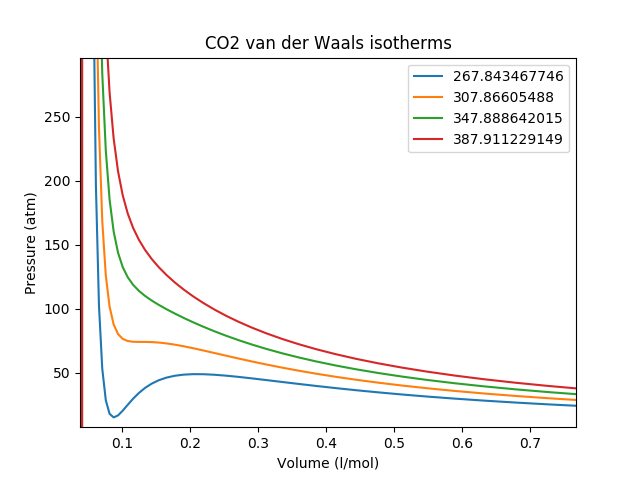
\includegraphics[width=.9\linewidth]{./figs/vdWgas.png}
\end{center}

\begin{center}
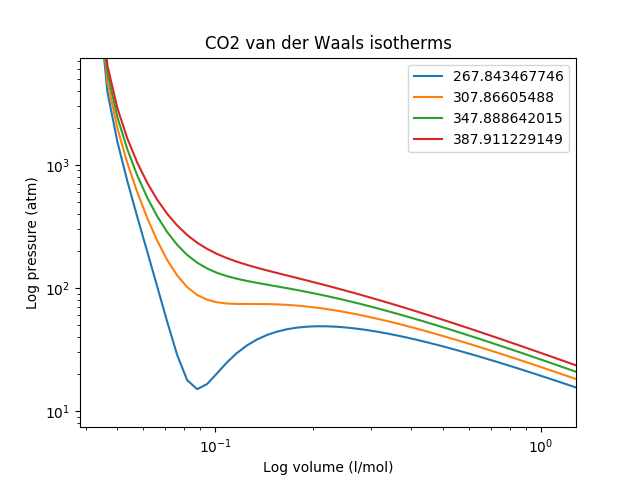
\includegraphics[width=.9\linewidth]{./figs/logvdWgas.png}
\end{center}

\subsection{Other thermodynamic potentials}
\label{sec:org589ecac}
\begin{enumerate}
\item Energy minimum principle minimum at constant entropy
\item Legendre transforms
\begin{enumerate}
\item \(Y=Y(X) \rightarrow \psi(P) = Y(P)-PX(P) \quad P=\partial Y /\partial X\)
\item \(P,\psi(P)\) give intercept and slope of tangents of \(Y\)
\end{enumerate}
\item Enthalpy \(H(S,P,N) = U + PV\)
\begin{enumerate}
\item Minimized at constant \(S\), \(P\), and \(N\)
\item Heat flow when only \(PV\) work done
\end{enumerate}
\item Helmholtz \(A(T,V,N) = U - TS\)
\begin{enumerate}
\item Minimized at constant \(T\), \(V\), and \(N\)
\item Maximum work from a process at temperature \(T\)
\end{enumerate}
\item Gibbs \(G(T,P,N) = U + PV - TS\)
\begin{enumerate}
\item Minimized at constant \(T\), \(P\), and \(N\)
\item Most useful for chemical problems
\item Gibbs-Helmholtz \(\left ( \dfrac{\partial (G/T)}{\partial T} \right )_{P,N} = -\dfrac{H}{T^2}\)
\end{enumerate}
\item Alles potential
\begin{enumerate}
\item Gibbs-Duhem redux
\end{enumerate}
\item Maxwell relations, see Table~\ref{Maxwell}.
\end{enumerate}
\subsection{Using thermodynamic potentials}
\label{sec:org9119ad9}
\begin{enumerate}
\item Using (differential) thermodynamic relations
\begin{enumerate}
\item Joule-Thompson effect
\end{enumerate}
\item Three unique susceptibilities of a one-component material (Table~\ref{susceptibilities})
\begin{enumerate}
\item All thermodynamic properties can be described in terms of the susceptibilities
\item Integrating susceptibilities
\item Heat capacity and departure functions
\end{enumerate}
\end{enumerate}
\begin{table}
  \begin{center}
  \caption{\label{Maxwell}Useful Maxwell Relationships}
  \begin{tabular}{ccc}
\hline
Enthalpy   & Helmholtz & Gibbs \\
 & & \\
$ \left ( \dfrac{\partial T}{\partial P}\right )_S =  \left ( \dfrac{\partial V}{\partial
    S}\right )_P  $ &
$ \left ( \dfrac{\partial S}{\partial V}\right )_T =  \left ( \dfrac{\partial P}{\partial
    T}\right )_S  $ &
$ \left ( \dfrac{\partial S}{\partial P}\right )_T =  -\left ( \dfrac{\partial V}{\partial
    T}\right )_P  $ \\
\hline
  \end{tabular}
  \end{center}
\end{table}
\begin{table}
  \begin{center}
  \caption{\label{susceptibilities}Susceptibilities}
  \begin{tabular}{cccc}
\hline
    Coefficient of thermal expansion & $\alpha$ &  $\dfrac{1}{v} \left (
      \dfrac{\partial v}{\partial T} \right )_P$  & $\dfrac{1}{v} \left (
      \dfrac{\partial^2 g}{\partial T \partial P} \right )_N$\\
  Isothermal compressibility   & $\kappa_T$  & $-\dfrac{1}{v} \left (
      \dfrac{\partial v}{\partial P} \right )_T$ & $-\dfrac{1}{v} \left (
      \dfrac{\partial^2 g}{\partial P^2} \right )_{T,N}$\\
  Constant  pressure heat capacity & $C_p$ & $ T \left ( \dfrac{\partial
      s}{\partial T}\right )_P $ & $-T \left (
      \dfrac{\partial^2 g}{\partial T^2} \right )_{P,N}$\\
  Constant  volume heat capacity & $C_v$ & $ T \left ( \dfrac{\partial
      s}{\partial T}\right )_v $ & \\
\hline
  \end{tabular}
  \end{center}
\end{table}

\subsection{Stability and phase equilibria}
\label{sec:orgcddbf7d}
\begin{enumerate}
\item Local stability condition
\begin{enumerate}
\item (Free) energy minimized \(dU=0\quad d^2U \geq 0\)
\item Entropy maximized \(dS = 0\quad d^2S \leq 0\)
\item Implies \(c_p \geq c_v \geq 0\), \(\kappa_T \geq \kappa_s \geq 0\)
\item Microscopic fluctuations and Le'Chatlier's principle
\end{enumerate}

\item Global stability conditions
\begin{enumerate}
\item Common tangents and convex hull
\item Lever rule
\item Phase separation---two phases have lower free energy
than one.  Balance of energetic attractions and entropic ``repulsion''
\item Critical points (\(d^3u = 0\)) attraction and repulsion
exactly in balance
\item Stable, metastable (spinodal), and unstable regions
\begin{enumerate}
\item Extensive quantities discontinuous between phases (``latent'' quantities)
\item Intensive quantities equal between phases
\item Susceptibilities discontinuous between phases
\end{enumerate}
\end{enumerate}

\item Gibbs-Duhem integrations
\item Equal area construction, \(d\mu = vdP\) along an isotherm
\item \(d\mu = - s dT\), chemical potential of each phase decreases with \(T\)
\item Phase diagrams---lines of equal chemical potential, \(\mu(l)=\mu(v)\)
\item Clausius equation
\begin{enumerate}
\item Along coexistence line \(dP/dT = \Delta s/\Delta v = \Delta
      h/T\Delta v\) in general
\item Clausius-Clapeyron for ideal vapor \(d\ln P/d(1/T) = -\Delta h/R\)
\end{enumerate}

\item Gibb's phase rule and triple point
\begin{enumerate}
\item \(DOF = c -\pi - R + 2\)
\end{enumerate}
\end{enumerate}

\section{The Microscopic View}
\label{sec:orgf96cf0d}
\subsection{Micro-canonical ensemble}
\label{sec:orgd76f5d1}
\subsubsection{Energy is \emph{quantized} at microscopic level}
\label{sec:org7537312}
\begin{enumerate}
\item Consequence of quantum mechanics
\item electronic, vibrational, rotational, translational
\item Need machinary to average QM information over macroscopic systems
\item Equal \emph{a priori} probabilities
\end{enumerate}
\subsubsection{Two-state model}
\label{sec:org29c16e9}
\begin{enumerate}
\item Box of particles, each of which can have energy 0 or \(\epsilon\)
\item Thermodynamic state defined by number of elements \(N\), and number of
quanta \(q\), \(U=q\epsilon\)
\item Degeneracy of given \(N\) and \(q\) given by binomial distribution:
\begin{displaymath}
  \Omega=\frac{N!}{q!(N-q)!}
\end{displaymath}
\item Allow energy to flow between two such systems
\begin{enumerate}
\item Energy of a closed system is conserved (first law!)
\item Degeneracy of total system is always \(\geq\) degeneracy of the
starting parts!
\item Boltzmann's tombstone, \(S = k_B \ln \Omega\)
\item Clausius: entropy of the universe seeks a maximum!  Second Law\ldots{}
\end{enumerate}
\item Energy flow/thermal equilibrium between two large systems
\begin{enumerate}
\item Each subsystem has energy \(U_i\) and degeneracy \(\Omega_i(U_i)\)
\item Bring in thermal contact, \(U=U_1+U_2\), \(\Omega=\Omega_1(U_1)\Omega_2(U_2)\)
\item If systems are very large, one combination of \(U_1\), \(U_2\) and \(\Omega\)
will be much more probably than all others
\item What value of \(U_1\) and \(U_2=U-U_1\) maximizes \(\Omega\)?
\end{enumerate}
\end{enumerate}
\begin{displaymath}
 \left ( \frac{\partial \ln \Omega_1}{\partial U_1} \right )_N = \left ( \frac{\partial \ln \Omega_2}{\partial U_2} \right )_N
\end{displaymath}
\begin{displaymath}
 \left ( \frac{\partial S_1}{\partial U_1} \right )_N = \left ( \frac{\partial S_2}{\partial U_2} \right )_N
\end{displaymath}
\begin{enumerate}
\item Thermal equilibrium is determined by equal \textbf{temperature!}
\begin{displaymath}
    \frac{1}{T}=\left ( \frac{\partial S}{\partial U} \right )_N
  \end{displaymath}
\begin{enumerate}
\item When the temperatures of the two subsystems are equal, the
entropy of the combined system is maximized!
\item (Same arguments lead to requirement that equal pressures (\(P_i\)) and
equal chemical potentials (\(\mu_i\)) maximize entropy when volumes or
particles are exchanged)
\end{enumerate}
\end{enumerate}

\subsubsection{Two-state model in limit of large \(N\)}
\label{sec:orgf29ccff}
\begin{enumerate}
\item Large \(N\) and Stirling's approximation
\item Fundamental thermodynamic equation of two-state system:
\begin{displaymath}
  S(U)=-k_B \left ( x \ln x + (1-x) \ln (1-x) \right ), \mathrm{where}\
  x = q/N = U/N\epsilon
\end{displaymath}
\item Temperature is derivative of entropy wrt energy yields
\begin{displaymath}
  U(T) = \frac{N\epsilon}{1+e^{\epsilon/k_BT}}
\end{displaymath}
\begin{enumerate}
\item \(T \rightarrow 0, U \rightarrow 0, S \rightarrow 0\), minimum disorder
\item \(T \rightarrow \infty, U \rightarrow N\epsilon/2, S \rightarrow
              k_B \ln 2\), maximum disorder
\end{enumerate}
\item Differentiate again to get heat capacity
\end{enumerate}

\subsection{Canonical ensemble}
\label{sec:orgb965107}
\subsubsection{Partition function}
\label{sec:org7895187}
\begin{enumerate}
\item Where do fundamental equations come from?
\item Direct construction of \(S(U)\) is generally intractable, so seek simpler approach
\item Imagine a system brought into thermal equilibrium with a much
larger ``reservoir'' of constant \(T\), such that the aggregate has a
total energy \(U\)
\item Degeneracy of a given system microstate \(j\) with energy \(U_j\)
is \(\Omega_{res}(U-U_j)\)
\begin{eqnarray*}
  T = \frac{dU_{res}}{k_Bd\ln\Omega_{res}} \\
  \Omega_{res}(U-U_j) \propto e^{-U_j/k_B T}
\end{eqnarray*}
\item Probability for system to be in a microstate with energy \(U_j\) given by Boltzmann
distribution!
\begin{displaymath}
  P(U_j) \propto e^{-U_j/k_B T} = e^{-U_j \beta}
\end{displaymath}
\item Partition function ``normalizes'' distribution, \(Q(T) = \sum_j
         e^{-U_j \beta}\)
\item For system of identical (distinguishable) elements with energy states \(\epsilon_i\),
can factor probability to show
\begin{eqnarray*}
  P(\epsilon_i) \propto e^{-\epsilon_i/k_B T} = e^{-\epsilon_i \beta},\
  \ \ \ \ \beta=1/k_BT
\end{eqnarray*}
\end{enumerate}

\subsubsection{Energy factoring}
\label{sec:org52b0b13}
\begin{enumerate}
\item If system is large, how to determine it's energy states \(U_j\)?  There
would be many, many of them!
\item One simplification is if we can write energy as sum of energies of
individual elements (atoms, molecules) of system:
\begin{align}
  U_j&=\epsilon_j(1)+\epsilon_j(2) + ... + \epsilon_j(N) \\
  Q(N,V,T) &= \sum_j e^{-U_j\beta} \\
  &=\sum_je^{-(\epsilon_j(1)+\epsilon_j(2) + ... + \epsilon_j(N))\beta}
\end{align}
\item \emph{If} molecules/elements of system can be distinguished from each
other (like atoms in a fixed lattice), expression can be factored:
   \begin{align}
     Q(N,V,T)&=\left ( \sum_j e^{-\epsilon_j(1)\beta}\right )\cdots \left ( \sum_j
       e^{-\epsilon_j(N)\beta}\right ) \\
   &= q(1)\cdots q(N) \\
   \text{Assuming all the elements are the same:}\\
   &= q^N \\
  q&=\sum_j e^{-\epsilon_j \beta}: \mathrm{molecular\ partition\ function}
\end{align}
\item \emph{If not} distinguishable (like molecules in a liquid or gas, or
electrons in a solid), problem is difficult, because identical
arrangements of energy amongst elements should only be counted once.
Approximate solution, good almost all the time:\}
\begin{equation}
  Q(N,V,T)=q^N/N!
\end{equation}
\item Sidebar: ``Correct'' factoring depends on whether individual elements are fermions or bosons, leads to funny things like superconductivity and superfluidity.
\end{enumerate}

\subsubsection{Two-state system again}
\label{sec:orgae8327c}
\begin{enumerate}
\item Partition function, \(q(T)=1+e^{-\epsilon\beta}\)
\item State probabilities
\item Internal energy \(U(T)\)
\begin{equation}
  U(T)=-N \left ( \frac{\partial \ln(1+e^{-\epsilon\beta})}{\partial\beta}
  \right)=\frac{N\epsilon e^{-\epsilon\beta}}{1+e^{-\epsilon\beta}}
\end{equation}
\item Heat capacity \(C_v\)
\begin{enumerate}
\item Minimum when change in states with \(T\) is small
\item Maximize when chagne in states with \(T\) is large
\end{enumerate}
\item Helmholtz energy, \(A= -\ln q/\beta\), decreasing function of \(T\)
\item Entropy
\item Distinguishable vs.$\backslash$ indistinguishable particles
\begin{enumerate}
\item Distinguishable (e.g., in a lattice): \(Q(N,V,T) = q(V,T)^N\)
\item Indistinguishable (e.g., a gas): \(Q(N,V,T)\approx q(V,T)^N/N!\)
\end{enumerate}
\item Thermodynamic functions in canonical ensemble
\end{enumerate}

\begin{table}\small
  \begin{center}
    \caption{Equations of the Canoncial ($NVT$) Ensemble}
    \label{Canonical}
    \begin{tabular}[h]{lccc}
      \hline
$\beta=1/k_BT$ & {\bf Full Ensemble} & {\bf Distinguishable particles} & {\bf Indistinguishable
particles} \\
               &               & (e.g. atoms in a lattice) & (e.g. molecules in
               a fluid) \\
\hline
Single particle & & & \\partition function& & $\displaystyle q(V,T) = \sum_i
e^{-\epsilon_i\beta} $& $\displaystyle q(V,T) = \sum_i e^{-\epsilon_i\beta} $ \\
Full partition & & & \\function & $\displaystyle Q(N,V,T) = \sum_j e^{-U_j\beta} $ &
$\displaystyle Q = q(V,T)^N $ & $\displaystyle Q = q(V,T)^N/N! $ \\
Log partition &  $\ln Q$ & $N\log q$ & $ N\ln q - \ln N! $\\
function & & & $\approx N(\ln Q - \ln N +1)$ \\ & & & \\
Helmholtz energy & $\displaystyle -\frac{\ln Q}{\beta}$ & $\displaystyle
-\frac{N\ln q}{\beta}$ & $\displaystyle -\frac{N}{\beta}\left (\ln\frac{q}{N} +
  1 \right ) $ \\
($A=U-TS$) & & & \\ & & &  \\
Internal energy ($U$)& $\displaystyle -\left (\frac{\partial\ln
    Q}{\partial\beta}\right )_{NV}$ & $\displaystyle -N\left (\frac{\partial\ln
    q}{\partial\beta}\right )_{V}$ &  $\displaystyle -N\left (\frac{\partial\ln
    q}{\partial\beta}\right )_{V}$ \\ & & & \\
Pressure ($P$) & $\displaystyle \frac{1}{\beta}\left (\frac{\partial\ln
    Q}{\partial V}\right )_{N\beta}$ & $\displaystyle \frac{N}{\beta}\left (\frac{\partial\ln
    q}{\partial V}\right )_{\beta}$ &  $\displaystyle \frac{N}{\beta}\left (\frac{\partial\ln
    q}{\partial V}\right )_{\beta}$ \\ & & & \\

Entropy ($S/k_B$) & $ \beta U + \ln Q$ & $\beta U + N \ln q$ & $\beta U +
N\left ( \ln(q/N) + 1\right )$ \\ & & & \\
Chemical potential ($\mu$) & $\displaystyle -\frac{1}{\beta}\left ( \frac{\partial \ln
    Q}{\partial N}\right )_{VT} $& $\displaystyle -\frac{\ln q}{\beta}$ & $\displaystyle
-\frac{\ln (q/N)}{\beta}$ \\ & & & \\
\hline
    \end{tabular}
{\bf NOTE!} All energies are referenced to their values at 0~K.  Enthalpy $H=U+PV$, Gibb's
Energy $G=A+PV$.
  \end{center}
\end{table}

\subsection{Ideal gases redux}
\label{sec:org926e5f6}
\subsubsection{Separability}
\label{sec:org006cc8d}
    \begin{displaymath}
      Q_{ig}(N,V,T) = \frac{(q_\mathrm{trans}q_\mathrm{rot}q_\mathrm{vib})^N}{N!}
\end{displaymath}

\subsubsection{Particle-in-a-box (translational states of a gas)}
\label{sec:org0bb1581}
\begin{enumerate}
\item Energy states \(\epsilon_n=n^2\epsilon_0, n=1,2, \ldots\),
\(\epsilon_0\) tiny for macroscopic \(V\)
\item \(\Theta_\mathrm{trans} = \epsilon_0/k_B\) translational temperature
\item \(\Theta_\mathrm{trans} << T \rightarrow\) \emph{many} states contribute
to \(q_\mathrm{trans}\rightarrow\) integral approximation
\begin{eqnarray*}
  q_\mathrm{trans,1D} = \int_0^\infty e^{-x^2\beta\epsilon_0}dx =
  L/\Lambda \\
  \Lambda = \left ( \frac{h^2\beta}{2\pi m} \right )^{1/2}\
  \mathrm{thermal\ wavelength} \\
  q_\mathrm{trans,3D} = V/\Lambda^3
\end{eqnarray*}
\item Internal energy
\item Heat capacity
\item Equation of state (!)
\item Entropy: Sackur-Tetrode equation
\end{enumerate}
\subsubsection{Rigid rotor (rotational states of a gas)}
\label{sec:orge31908c}
\begin{enumerate}
\item energy states and degeneracies
\item \(\Theta_\mathrm{rot} = \hbar^2/2 I k_B\)
\item ``High'' T \(q_\mathrm{rot}(T) \approx \sigma \Theta_\mathrm{rot}/T\)
\end{enumerate}
\subsubsection{Harmonic oscillator (vibrational states of a gas)}
\label{sec:org73ddfa2}
\begin{enumerate}
\item \(\Theta_\mathrm{vib}=h\nu/k_B\)
\end{enumerate}
\subsubsection{Electronic partition functions \(\rightarrow\) spin multiplicity}
\label{sec:orga2b5a1e}
\subsubsection{Solids}
\label{sec:orgcd83ca4}
\begin{enumerate}
\item Equipartition
\item Law of Dulong and Petitt
\item Einstein crystal and heat capacity
\item Debye crysal
\end{enumerate}

\begin{table}
\begin{center}
    \caption{\large{Statistical Thermodynamics of an Ideal Gas}}
   \begin{description}
    \item[\underline{Translational DOFs}] {3-D particle in a box model}

$\displaystyle \theta_\mathrm{trans}= \frac{\pi^2\hbar^2}{2 m
  L^2 k_B}$,
$\displaystyle \Lambda=h\left( \frac{\beta}{2\pi m}\right )^{1/2}$

For $ T >> \Theta_\mathrm{trans}$, $\Lambda << L$, $\displaystyle
q_\mathrm{trans}=V/\Lambda^3$ (essentially always true)

\begin{tabular}{ccc}
$\displaystyle U_\mathrm{trans}=\frac{3}{2}RT$ & $\displaystyle C_\mathrm{v,trans} =
\frac{3}{2}R $ & $\displaystyle S^\circ_\mathrm{trans}=R \ln \left (
  \frac{e^{5/2}V^\circ}{N^\circ \Lambda^3}\right ) = R \ln \left (
  \frac{e^{5/2}k_BT}{P^\circ \Lambda^3}\right ) $ \\
\end{tabular}

  \item[\underline{Rotational DOFs}] {Rigid rotor model}
\begin{description}
\item[Linear molecule]{}
$\theta_\mathrm{rot} =hcB/k_B$

\begin{equation*}
q_\mathrm{rot}=\frac{1}{\sigma}\sum_{l=0}^\infty (2l+1)e^{-l(l+1)\theta_\mathrm{rot}/T},
\approx \frac{1}{\sigma}\frac{T}{\theta_\mathrm{rot}},\ \ T>>\theta_\mathrm{rot}\ \ \ \sigma = \left \{
        \begin{array}{rl}
          1, & \text{unsymmetric} \\
          2, & \text{symmetric}
        \end{array} \right .
\end{equation*}
\begin{tabular}{ccc}
$\displaystyle U_\mathrm{rot}=RT$ & $\displaystyle C_\mathrm{v,rot} =
R $ & $\displaystyle S^\circ_\mathrm{rot}=R (1-\ln(\sigma\theta_\mathrm{rot}/T)) $ \\
\end{tabular}

\item[Non-linear molecule]{} $\theta_{\mathrm{rot},\alpha}=hcB_\alpha/k_B$
\begin{equation*}
q_\mathrm{rot}
\approx \frac{1}{\sigma}\left ( \frac{\pi
    T^3}{\theta_{\mathrm{rot},\alpha}\theta_{\mathrm{rot},\beta}\theta_{\mathrm{rot},\gamma}}
  \right )^{1/2},\ \ T>>\theta_{\mathrm{rot},\alpha,\beta,\gamma}\ \ \ \sigma =
  \text{rotational symmetry number}
\end{equation*}
\begin{tabular}{ccc}
$\displaystyle U_\mathrm{rot}=\frac{3}{2}RT$ & $\displaystyle C_\mathrm{v,rot} = \frac{3}{2}
R $ & $\displaystyle S^\circ_\mathrm{rot}=\frac{R}{2}
\left ( 3-\ln\frac{\sigma\theta_{\mathrm{rot},\alpha}\theta_{\mathrm{rot},\beta}\theta_{\mathrm{rot},\gamma}}{\pi
  T^3} \right ) $ \\
\end{tabular}

\end{description}

\item[\underline{Vibrational DOFs}] {Harmonic oscillator model}
\begin{description}
\item[Single harmonic mode] {$\theta_\mathrm{vib}=h\nu/k_B $}
  \begin{equation*}
    q_\mathrm{vib}=\frac{1}{1-e^{-\theta_\mathrm{vib}/T}} \approx
      \frac{T}{\theta_\mathrm{vib}}, \ \ \ T>>\theta_\mathrm{vib}
  \end{equation*}

\begin{tabular}{ccc}
$ U_\mathrm{vib}= $ & $  C_\mathrm{v,vib} = $ & $S^\circ_{\mathrm{vib},i}=$ \\
$\displaystyle
R\frac{\theta_\mathrm{vib}}{e^{\theta_\mathrm{vib}/T}-1}$ &
$\displaystyle R\left (
  \frac{\theta_\mathrm{vib}}{T}\frac{e^{\theta_\mathrm{vib}/2T}}{e^{\theta_\mathrm{vib}/T}-1}
\right )^2 $ & $\displaystyle R \left ( \frac{\theta_\mathrm{vib}/T}{e^{\theta_\mathrm{vib}/T}-1}
-\ln(1-e^{-\theta_\mathrm{vib}/T})\right ) $ \\
\end{tabular}

\item[Multiple harmonic modes] {$\theta_{\mathrm{vib},i}=h\nu_i/k_B $}

  \begin{equation*}
    q_\mathrm{vib}=\prod_i\frac{1}{1-e^{-\theta_{\mathrm{vib},i}/T}}
  \end{equation*}

\begin{tabular}{ccc}
$ U_\mathrm{vib}= $ & $  C_\mathrm{v,vib} = $ & $S^\circ_{\mathrm{vib},i}=$ \\
$\displaystyle
R\sum_i\frac{\theta_{\mathrm{vib},i}}{e^{\theta_{\mathrm{vib},i}/T}-1}$ &
$\displaystyle R \sum_i \left (
  \frac{\theta_{\mathrm{vib},i}}{T}\frac{e^{\theta_{\mathrm{vib},i}/2T}}{e^{\theta_{\mathrm{vib},i}/T}-1}
\right )^2 $ & $\displaystyle R \left ( \frac{\theta_{\mathrm{vib},i}/T}{e^{\theta_{\mathrm{vib},i}/T}-1}
-\ln(1-e^{-\theta_{\mathrm{vib},i}/T})\right ) $ \\
\end{tabular}

\end{description}
\item[\underline{Electronic DOFs}] {}
$q_\mathrm{elec} = \text{spin multiplicity}$

\end{description}
\end{center}
\end{table}

\begin{table}
  \begin{center}
    \caption{\large{Contributions of Molecular Degrees of Freedom to Gas Thermodynamics}}
    \begin{tabular}{lcccc}
\hline \\
{\bf DOF}  & {\bf Characteristic} & {\bf Characteristic} & {\bf \#states at} & {\bf Internal }\\
        & {\bf energy}  & {\bf temperature} & {\bf $\approx 300$~K} & {\bf energy }\\
\hline \\
Translational & $\epsilon_\mathrm{trans} = \frac{\hbar^2}{2mL^2} \approx 10^{-21} \mathrm{cm}^{-1} $ &
$\theta_\mathrm{trans} \approx 10^{-21}$~K & $\approx 10^{30}$ & $U= \frac{3}{2}RT $  \\ \\
Rotational & $\epsilon_\mathrm{rot} \approx 1~\mathrm{cm}^{-1}$ & $\theta_\mathrm{rot} \approx 1$~K &
$\approx 100s$ & $\approx \mathrm{\#DOF}\cdot RT $\\ \\
Vibrational & $\epsilon_\mathrm{vib} \approx 1000~\mathrm{cm}^{-1} $ & $\theta_\mathrm{vib} \approx
1000$~K & $\approx 1$ & non-classical, $0\rightarrow RT$ \\ \\
Electronic & $\epsilon_\mathrm{elec} \approx 10000~\mathrm{cm}^{-1} $ & $\theta_\mathrm{elec} \approx
10000$~K & $\approx 1$ & 0\\
\hline
    \end{tabular}
\begin{eqnarray*}
Q = \left ( q_\mathrm{trans} q_\mathrm{rot} q_\mathrm{vib} q_\mathrm{elec} \right )^N/N! \\
 \\
U = U_\mathrm{trans} + U_\mathrm{rot} + U_\mathrm{vib} + U_\mathrm{elec}, \ldots
\end{eqnarray*}
  \end{center}

\end{table}

\subsubsection{Other ensembles}
\label{sec:org086bc34}
\begin{enumerate}
\item Isothermal/isobaric
\begin{enumerate}
\item \(\Delta(T,P,N) = \sum_j e^{-U_j\beta} e^{-PV_j\beta}\)
\item \(G(T,P,N) = -k_B T \ln \Delta(T,P,N)\)
\end{enumerate}
\item Grand canonical
\begin{enumerate}
\item \(\Xi(T,V,\mu) = \sum_j e^{-U_j\beta} e^{-PV_j\beta}e^{\mu N_j \beta}\)
\item \(\Psi(T,V,\mu) = - k_B T \ln \Xi(T,V,\mu)\)
\item Langmuir isotherm example
\end{enumerate}
\end{enumerate}
\section{Thermodynamics of Stuff}
\label{sec:org39be236}
\subsection{Theory of non-ideal fluids}
\label{sec:org6ae7146}
\subsubsection{Non-ideality}
\label{sec:orgde7aa9a}
\begin{enumerate}
\item Real molecules interact through vdW interactions
\begin{enumerate}
\item dipole-dipole, dipole-induced dipole, induced dipole-induced dipole
(London dispersion)
\item scale with dipole moments(\(\vec{\mu}\) and polarizability volumes
(\(\alpha\)) of molecules
\item \(U(r) \approx - c/r^6\)
\end{enumerate}
\item Particle-in-a-box model breaks down, have to work harder but
can still get at same ideas
\item Configurational integral \(Q_\mathrm{config}=\int \ldots \int e^{-U(r)\beta} dr_1\ldots dr_n\)
\end{enumerate}
\subsubsection{van der Waals gas}
\label{sec:org45d3228}
\begin{enumerate}
\item Hard sphere + \(1/r^6\) potential + mean-field approximation (\(g(r)=1\))
\item \(Q_\mathrm{config} = ((V-Nb) \exp (-(\phi/2)\beta))^N \rightarrow\) vdW EOS
\item See Hill, \emph{J. Chem. Ed.} \textbf{1948}, \emph{25}, 347, \url{http://dx.doi.org/10.1021/ed025p347}
\item Free energy has two competing contributions
\item \(f_\text{vdW} = - k_BT \ln \{ (v-b)(k_BT)^{3/2}\} -a/v -k_BT\)
\item \(P_\text{vdW}=RT/(v-b) - a/v^2\)
\end{enumerate}

\subsubsection{Radial distribution functions, \(g(r)\), for gases, liquids, solids}
\label{sec:org932b967}
\subsubsection{Virial expansion}
\label{sec:org7b0a46a}
\begin{enumerate}
\item Configurational integral can be expanded in powers of \(1/v\) times ``virial''
coefficients \(B_j(T)\)
\item \(f(T,P) = f_\text{ig}(T,P) - RT \{ B_2(T)/v + B_3(T)/v^2 + \ldots \}\)
\item \(Z = 1 + B_2(T)/v + B_3(T)/v^2 + \dots\)
\item ``Second'' virial coefficient \(B_2(T)\) limiting low density ``departure'' of
volume from that of an ideal gas, \(v_\text{res}(T,v) = v -
     v_\text{ig}=(RT/P)(Z-1)\)
	\[B_2(T) = \lim_{v \rightarrow \infty} v_\text{res}, \]
\begin{itemize}
\item Virial coefficients integrate ``clusters'' of intermolecular interactions, 2-body, 3-body, \(\ldots\)
\end{itemize}
\item \(B_2(T) = -2\pi N_A \int_0^\infty \{e^{-u(r)/k_BT}-1\}r^2dr\)
\item \(B_2^\text{vdW} (T) = b -a/RT\)
\item Lennard-Jones potential
\end{enumerate}

\subsubsection{Modern approach is to use numerical methods}
\label{sec:orgd56a107}
\begin{enumerate}
\item ``forcefield'' to represent intra- and intermolecular properties
\item molecular dynamics or Monte Carlo to sample interactions
\item Fluid property challenge at AIChE
\end{enumerate}

\subsection{Engineering representations of fluids}
\label{sec:org09a5cad}
\subsubsection{How to represent properties of real fluids?}
\label{sec:org91c2dec}
\begin{enumerate}
\item Mechanical equations of state (empirical)
\item Thermodynamic tabulations (JANAF, steam tables)
\item Theoretical models (virial expansion)
\item Computer simulations (molecular interactions)
\end{enumerate}

\subsubsection{Thermodynamic integrations}
\label{sec:org76ee34d}
\begin{enumerate}
\item Integrate susceptibilities
\item Integrate \(PvT\) relationship plus \(C_p^{ig}(T)\)
\end{enumerate}

\subsubsection{Compressibility}
\label{sec:org3f0c5f5}
\begin{enumerate}
\item Fluids deviate from ideality because they have finite size and interact over distances, origin of two-parameter EOS
\item Compressibility \(Z(T,P)=P/P^{ig}=Pv/RT\) measures deviation from ideality
\item Critical compressibility \(Z_c \approx 0.27\) for all ``normal'' fluids
\item Reduced variable \(T_R=T/T_c\), \(P_R = P/P_c\), \(v_R = v/v_c\)
\item ``Law'' of corresponding states---all ``normal'' fluids have the same \(PvT\) behavior in reduced variables
\item Allows fluids to be described on generalized compressibility chart
\end{enumerate}

\subsubsection{Cubic mechanical equations of state}
\label{sec:org1d8156d}
\begin{enumerate}
\item van der Waals, \(Z_c = 0.375\)
\item Redlich-Kwong,  \(Z_c = 0.333\)
\item Peng-Robinson, \(Z_c = 0.307\)
\item Empirically parameterized, all obey law of corresponding states, none perfect
\end{enumerate}
\subsubsection{Departure functions measure thermodynamic potential difference between real}
\label{sec:orgf4d3ef9}
state and hypothetical ``ideal gas'' state
\begin{enumerate}
\item \(\Delta\)whatever = \(\Delta\) ideal + \(\Delta\) departure
\item From generalized compressibility or accurate EOS integration
\item Entropy departure \(s(T,P) - s^{ig}(T,P) = R \ln Z(T,P) + \int_\infty^{v(T,P)} \left [ \left ( \frac{\partial P}{\partial T}\right )_v - \frac{R}{v} \right ] dv\)
\item Enthalpy departure \(h(T,P) - h^{ig}(T,P) = RT \left ( Z-1 \right )  + \int_\infty^{v(T,P)} \left [ T \left  ( \frac{\partial P}{\partial T}\right )_v - P \right ] dv\)
\end{enumerate}
\subsubsection{Fugacity measures departure of free energy ideality}
\label{sec:orgb775f03}
\begin{enumerate}
\item Define \(\mu(T,P) = \mu^\circ(T) + RT \ln f(T,P)/f^\circ(T)\)
\begin{equation*}
  \lim_{P\rightarrow 0} \mu = -\infty\quad \lim_{P\rightarrow 0} f =P^\text{ig} =0
\end{equation*}
\begin{equation*}
  \ln f/P = \dfrac{RT}{P}\int_0^P(Z-1)dP
\end{equation*}
\item \(\mu^\alpha = \mu^\beta\) implies \(f^\alpha = f^\beta\).
\item Fugacity coefficient \(\gamma(T,P) = f(T,P)/P\)
\begin{equation*}
  \ln\gamma=\int_o^P\dfrac{Z-1}{P}dP
\end{equation*}
\end{enumerate}
\subsection{Single-phase mixtures}
\label{sec:org092eb9d}
\subsubsection{Ideal gas mixtures}
\label{sec:orge9de7aa}
\begin{enumerate}
\item Statistical mechanical approach
\item Properties of ideal mixture
\begin{equation*}
  \Delta u_\text{mix} = \Delta v_\text{mix} = 0 \qquad \Delta s_\text{mix} = - k_B \sum_i y_i \ln y_i
\end{equation*}
\item Partial pressure \(P_i = y_i P\)
\item Chemical potential \(\mu_i(y_i,T) = \mu_i^\circ(T) + k_B T \ln \left ( y_i
              P/P^\circ \right)\)
\item Work of separation and Gibbs paradox
\end{enumerate}

\subsubsection{Non-ideal gas mixtures}
\label{sec:org317682c}
\begin{enumerate}
\item Inconvenient that \(\lim_{y_{i}\to 0}\mu_i(y_i,T,P) = -\infty\)
\item Construct \emph{fugacity} to obey same equilibrium conditions as chemical potential but to tend to \(y_{i}P\) in infinite dilution
\begin{equation*}
  \bar{f}_i(y_{i},T,P) = P^{\circ} \exp \left [ (\mu_i(y_i,T,P) - \mu_i^\circ(T))/ k_B T \right ]
\end{equation*}
\item Chemical potential \(\mu_i(y_i,T,P) = \mu_i^\circ(T) + k_B T \ln \left ( /P^\circ \right)\)
\item Fugacity coefficient \(\phi_{i}(y_{i,T,P})=\bar{f}_{i}(y_{i},T,P)/(y_{i}P)\)
\item Fugacity can be computed from a mixture-explicit EOS
\begin{equation*}
	    R T \ln \left ( \bar{f}_i/y_i P \right ) = \int_0^P \left (
      \bar{v}_i - \frac{RT}{P} \right ) dP  =  \frac{1}{RT} \left ( \frac{\partial (F - F^\text{ig})}{\partial N_i} \right )_{T,V,N_{j\neq i}} - \ln Z
 \end{equation*}
\item Virial mixture equation, vdW equation, \ldots
\item Lorentz-Berthelot mixing
\begin{equation*}
  b = \sum_i b_i \qquad a = \sum_i\sum_j y_i y_j a_{ij} \qquad a_{ij} = \sqrt{a_ia_j}
\end{equation*}
\item Lewis (ideal) fugacity rule \(\bar{f}_i \approx y_i f_i\) generalization of ideal gas
\end{enumerate}
\subsubsection{Ideal liquid mixtures}
\label{sec:org5e23ba2}
\begin{enumerate}
\item Lattice model with random distribution of molecules

\begin{equation*}
\Delta u_\text{mix} = \Delta v_\text{mix} = 0 \qquad \Delta s_\text{mix} = - k_B \sum_i x_i \ln x_i
\end{equation*}
\begin{equation*}
\mu_i(x_i,T) = \mu_i^\circ(T) + k_B T \ln \left ( x_i \right)
\end{equation*}

\item True for liquids of comparable molecular dimensions and interactions
\end{enumerate}
\subsubsection{Partial molar quantities}
\label{sec:orge9e2b48}
\begin{enumerate}
\item For any extensive quantity or susceptibility, \(J\):
     \begin{equation*}
\bar{J}_i = \left ( \frac{\partial J}{\partial N_i} \right )_{N_{j\neq i}}
     \qquad J = \sum_i \bar{J}_i N_i \qquad j = \sum \bar{J}_i x_i
     \end{equation*}
\begin{equation*}
\Delta j_\text{mix} = \sum_i \bar{J}_ix_i - \sum_i j_i x_i
\end{equation*}
\item Gibbs-Duhem says partial molar properties are not independent: \(\sum_i N_i d\bar{J}_i = 0\)
\end{enumerate}

\subsubsection{Non-ideal liquid mixtures}
\label{sec:orgb4ff18f}
\begin{enumerate}
\item Bragg-Williams/mean field approximation
\item Differential exchange parameter \(\chi_{AB}\)

\begin{equation*}
   \chi_{12} = \frac{z}{k_BT}\left ( u_{12} - \frac{u_\text{11} +
    u_\text{22}}{2} \right )
\end{equation*}

\item Hildebrand regular solution and excess mixing quantities
\begin{equation*}
   \Delta g_\text{xs}/k_BT = \chi_{12} x_1(1-x_2)
\end{equation*}
\begin{equation*}
    \mu_1(T,x_1) = \mu_1^\text{ideal}(T,x_1) + k_B T \chi_{12} (1-x_1)^2
\end{equation*}
\item Activity and activity coefficient
\begin{enumerate}
\item Solvent convention
\item Solute convention
\end{enumerate}
\item Liquid-liquid phase diagrams
\begin{enumerate}
\item Phase separation, critical point
\end{enumerate}
\item Freezing point depression/boiling point elevation
\end{enumerate}
\subsubsection{Ionic mixtures}
\label{sec:org6938dd3}
\begin{enumerate}
\item Debye-Huckel
\end{enumerate}

\subsection{Gas-liquid equilibria}
\label{sec:orgda4c665}
\subsubsection{Ideal-ideal liquid-vapor mixtures}
\label{sec:orgf0e8816}
\begin{enumerate}
\item Equal chemical potentials in each phase
\item Equilibrium cycle (relate to single component phase equilibrium): start from single component l-v equilibrium, compress each component to desired pressure, then mix.
\item Gas compression important, liquid compression (Poynting correction) less so.
\item Ideal vapor-liquid equilibrium \(\rightarrow\) Raoult's Law:
\begin{equation*}
  \mu_i^\text{gas} = \mu_i^\text{liq} \rightarrow y_i P = x_i P_i^*
\end{equation*}
\item Pressure-composition diagram
\item Temperature-composition diagram
\end{enumerate}

\subsubsection{Non-ideal liquid/ideal vapor}
\label{sec:org7f729c1}
\begin{enumerate}
\item Regular solution
   \begin{equation*}
  \chi_{12} \left \{
   \begin{array}{rl}
     > 0 & \text{positive deviation from Raoult's Law,}\\
     = 0 & \text{Raoult's Law,}\\
     <0 & \text{negative deviation from Raoult's Law}
    \end{array} \right .
\end{equation*}
\item Temperature-composition diagrams
\begin{enumerate}
\item Liquid-vapor
\item Eutectics, \ldots{}
\end{enumerate}
\item Henry's Law (dilute) limit
\item Gibbs-Duhem consequences
\end{enumerate}


\section{Thermodynamics of Change}
\label{sec:orgc237df3}
\subsection{Chemical thermodynamics and equilibria}
\label{sec:org61ba7eb}
\begin{enumerate}
\item Chemical reactions
\item Thermodynamic potential differences
\begin{enumerate}
\item Standard states
\item Reaction entropy \(\Delta S^\circ (T) =  S^\circ_\mathrm{B}(T)-S^\circ_\mathrm{A}(T)\)
\item Reaction energy \(\Delta U^\circ (T) = U^\circ_\mathrm{B}(T)-U^\circ_\mathrm{A}(T)+\Delta E(0)\)
\item Gibbs-Helmholtz
\end{enumerate}
\item Equilibrium-closed system
\begin{enumerate}
\item Equilibrium constants and algebraic solutions
\item Free energy minimization
\item Parallel reactions
\end{enumerate}
\item Equilibrium-open system
\begin{enumerate}
\item Reaction phase diagrams
\end{enumerate}
\item Partition functions and \(K_{eq}\)
\item Non-ideal activities
\item Electrochemical reactions
\end{enumerate}

\begin{table}
\begin{center}
    \caption{\large{Equilibrium and Rate Constants}}
   \begin{description}
   \item[Equilibrium Constants] $a~\text{A} + b~\text{B} \rightleftharpoons c~\text{C} + d~\text{D} $
     \begin{eqnarray*}
       K_{eq}(T) &=& e^{\Delta S^\circ(T,V)/k_B}e^{-\Delta H^\circ(T,V)/k_BT}
       \\ \\
            K_c(T) &=&
           \left(\frac{1}{c^\circ}\right)^{\nu_c+\nu_d-\nu_a-\nu_b}\frac{(q_c/V)^{\nu_c}(q_d/V)^{\nu_d}}{(q_a/V)^{\nu_a}(q_b/V)^{\nu_b}}e^{-\Delta
            E(0)\beta}\\ \\
            K_p(T) &=&
          \left(\frac{k_BT}{P^\circ}\right)^{\nu_c+\nu_d-\nu_a-\nu_b}\frac{(q_c/V)^{\nu_c}(q_d/V)^{\nu_d}}{(q_a/V)^{\nu_a}(q_b/V)^{\nu_b}}e^{-\Delta
            E(0)\beta}
\end{eqnarray*}
\item[Unimolecular Reaction] $\text[A] \rightleftharpoons [\text{A} ]^\ddagger
  \rightarrow C$
      \begin{displaymath}
        k(T)=\nu^\ddagger \bar K^\ddagger=\frac{k_B T}{h} \frac{\bar{q}_\ddagger(T)/V}{q_A(T)/V}
          e^{-\Delta E^\ddagger(0)\beta}
      \end{displaymath}
\begin{center}
      \begin{tabular}{cc}
      $ \displaystyle E_a =\Delta H^{\circ\ddagger}+k_B T $
      & $ \displaystyle A = e^1\frac{k_B T}{h} e^{\Delta S^{\circ\ddagger}} $
      \end{tabular}
\end{center}
\item[Bimolecular Reaction] $
        \mathrm{A} + \mathrm{B} \rightleftharpoons [ \mathrm{AB}]^\ddagger
        \rightarrow \text{C}$
      \begin{displaymath}
        k(T)=\nu^\ddagger \bar K^\ddagger=\frac{k_B T}{h} \frac{q_\ddagger(T)/V}{(q_A(T)/V)(q_B(T)/V)}\left
          (\frac{1}{c^\circ}\right )^{-1}
        e^{-\Delta E^\ddagger(0)\beta}
      \end{displaymath}
      \begin{center}
        \begin{tabular}{cc}
        $ \displaystyle E_a  =\Delta H^{\circ\ddagger}+2 k_B T $ & $ \displaystyle
        A  = e^2\frac{k_B T}{h} e^{\Delta S^{\circ\ddagger}} $
      \end{tabular}
      \end{center}
   \end{description}
 \end{center}
 \end{table}

\subsection{Non-equilibrium thermodynamics}
\label{sec:org2658aed}
\begin{table}
\begin{center}
\caption{Physical units}
\begin{tabular}{|lrlrl|}
  \hline
  $N_\mathrm{Av}$: & $6.02214 \times 10^{23}$& mol$^{-1}$  & & \\
  1 amu: & $1.6605\times 10^{-27}$ & kg & & \\
  $k_\mathrm{B}$: & $1.38065\times 10^{-23}$ & J~K$^{-1}$ & $8.61734\times
  10^{-5}$ & eV K$^{-1}$\\
  $R$: & 8.314472 & J K$^{-1}$ mol$^{-1}$ & $8.2057 \times 10^{-2}$ & l atm mol$^{-1}$ K$^{-1}$\\
  $\sigma_\mathrm{SB}$: & $5.6704\times 10^{-8}$ & J s$^{-1}$ m$^{-2}$ K$^{-4}$ & & \\
  $c$: & $2.99792458\times 10^8$ & m s$^{-1}$ & & \\
  $h$: & $6.62607\times 10^{-34}$ & J s & $4.13566\times 10^{-15}$ & eV s
  \\
  $\hbar$: & $1.05457\times 10^{-34}$ & J s & $6.58212\times 10^{-16}$&  eV s \\
  $hc$: & 1239.8 & eV nm  & & \\
  $e$: & $1.60218\times 10^{-19}$ &  C & & \\
  $m_e:$ & $9.10938215\times 10^{-31}$ & kg &0.5109989 & MeV c$^{-2}$  \\
  $\epsilon_0$: & $8.85419 \times 10^{-12}$ & C$^2$ J$^{-1}$ m$^{-1}$ & $5.52635\times
  10^{-3}$ & $e^2$ \AA$^{-1}$ eV$^{-1}$ \\
  $e^2/4\pi\epsilon_0$: & $2.30708 \times 10^{-28}$&  J m & 14.39964 & eV \AA\\
  $a_0$: & $0.529177 \times 10^{-10}$ & m & 0.529177 & \AA\\
  $E_\mathrm{H} $: & 1 & Ha & 27.212 & eV \\
  \hline
\end{tabular}
\end{center}
\end{table}
\end{document}